\chapter{Complex Bands and Non-Hermitian Gaps}
\label{ch:complex-bands}

\begin{chapterlead}
In Hermitian photonic crystals, a band gap is a frequency window with no
propagating modes. In non-Hermitian crystals, eigenfrequencies are
complex, and the very notion of a ``gap'' must be rethought. Two
fundamentally different gap structures emerge---the \emph{line gap} and
the \emph{point gap}~\cite{kawabata2018symmetry,kawabata2019classification,ryu2010topological}---each supporting its own class of topological
invariants. The theory of complex photonic bands is developed by
introducing the two gap types with concrete examples, deriving the spectral
winding number from the complex band dispersion, and showing how the
biorthogonal Berry phase~\cite{yao2018edge,yokomizo2019non,kunst2018biorthogonal,icon2021exceptional,shen2017topological,gong2018topological} generalizes the Hermitian topological framework
to non-Hermitian systems.
\end{chapterlead}


%% ================================================================
\section{From real to complex band structure}
\label{sec:complex-bands-intro}

When the permittivity of a periodic photonic crystal acquires an imaginary
part---through material loss, gain, or radiation coupling---the Bloch
eigenproblem of Chapter~\ref{ch:periodicity} still admits solutions
labeled by $\kk$ (Bloch's theorem depends on translational symmetry, not
Hermiticity), but the eigenfrequencies become complex:
\begin{equation}
 \omega_n(\kk) = \omega_n'(\kk) + i\omega_n''(\kk).
 \label{eq:complex-band}
\end{equation}
The ``band structure'' is now a set of curves in the three-dimensional
space $(\kk, \Re\omega, \Im\omega)$, or equivalently a set of trajectories
in the complex $\omega$ plane as $\kk$ sweeps the Brillouin zone.

\subsection{How complex bands arise from Maxwell equations}
\label{ssec:complex-bands-maxwell}

The passage from real to complex bands can be understood directly from
the Maxwell eigenproblem. In a lossless periodic medium
($\Im\epsr = 0$), the operator
$\hat{\Theta}_\kk = \epsr^{-1}\curl(\mur^{-1}\curl\,\cdot\,)$ acting on
Bloch-periodic fields is self-adjoint in the $\epsr$-weighted inner
product. Its eigenvalues $\omega_n^2(\kk)/c^2$ are real and positive.

When $\Im\epsr \neq 0$, the operator ceases to be self-adjoint, and its
eigenvalues become complex. The imaginary part of the eigenfrequency
has a clear physical meaning from the energy balance:
\begin{equation}
 \omega_n''(\kk) \approx -\frac{\omega_n'(\kk)}{2}
 \frac{\int_{\mathrm{uc}} \Im\epsr(\rr)\,|\mathbf{u}_{n\kk}(\rr)|^2\;\dd^d r}
 {\int_{\mathrm{uc}} \Re\epsr(\rr)\,|\mathbf{u}_{n\kk}(\rr)|^2\;\dd^d r},
 \label{eq:omega-imag-perturbation}
\end{equation}
valid to first order in $\Im\epsr$. Modes concentrated in lossy regions
($\Im\epsr > 0$) acquire $\omega_n'' < 0$ (decay); modes in gain
regions ($\Im\epsr < 0$) acquire $\omega_n'' > 0$ (amplification).
Different Bloch modes at the same $\kk$ sample the gain/loss distribution
differently, so they can have imaginary parts with different signs and
magnitudes.

\subsection{Consequences of complexification}
\label{ssec:complex-consequences}

This complexification has immediate consequences:
\begin{itemize}
 \item Bands can no longer be ordered by frequency along the real axis;
 two bands may cross in $\Re\omega$ while being separated in
 $\Im\omega$, or vice versa.
 \item The concept of a ``gap'' must specify what it means for two
 complex-valued curves to be ``separated.''
 \item Exceptional points---where both eigenvalues and eigenvectors
 coalesce (Chapter~\ref{ch:exceptional-points})---can appear as
 singular points in the $(\kk, \omega)$ space.
 \item The standard bulk-boundary correspondence, which relates the
 Chern number to edge-state counts, may fail because the bulk
 invariant was defined assuming a real spectrum
 (Chapter~\ref{ch:bbc-rebuilt}).
\end{itemize}

\subsection{A concrete example: 1D gain--loss lattice}
\label{ssec:1d-example}

Consider a one-dimensional tight-binding model with alternating on-site
gain and loss:
\begin{equation}
 H(k) = \begin{pmatrix} i\gamma & t(1+e^{-ik}) \\
 t(1+e^{ik}) & -i\gamma \end{pmatrix},
 \label{eq:gain-loss-ssh}
\end{equation}
where $t$ is the hopping and $\gamma$ is the gain/loss rate. This is
an SSH model with a $\PT$-symmetric non-Hermitian perturbation. The
eigenvalues are
\begin{equation}
 \omega_\pm(k) = \pm\sqrt{4t^2\cos^2(k/2) - \gamma^2}.
 \label{eq:gl-ssh-eigenvalues}
\end{equation}
For any nonzero $\gamma$, momenta close to $k=\pi$ satisfy
$|2t\cos(k/2)|<|\gamma|$, so the square root is imaginary and the
corresponding Bloch states are in a $\PT$-broken sector. Momenta farther
from $k=\pi$ remain real when $|2t\cos(k/2)|>|\gamma|$. Thus this
balanced gain--loss dimer is useful for illustrating complex bands and
exceptional points, but it is not by itself the canonical point-gap
skin-effect model. For point-gap topology and skin effect one needs
non-reciprocal hopping, as in the Hatano--Nelson or asymmetric SSH
models discussed below~\cite{gong2018topological,shen2017topological}.

\paragraph{Perturbation theory for complex bands.}
The first-order imaginary shift~\eqref{eq:omega-imag-perturbation} can
be made concrete for this lattice. At $k = 0$ the Bloch modes of the
unperturbed SSH model are $|u_\pm\rangle = (1,\;\pm 1)^\transpose/\sqrt{2}$
with $\omega_\pm(0) = \pm 2t$. The gain--loss perturbation
$\delta H = i\gamma\,\sigma_z$ has matrix elements
\begin{equation}
 \langle u_\pm | \delta H | u_\pm \rangle = 0,
 \qquad
 \langle u_\pm | \delta H | u_\mp \rangle = \pm i\gamma.
 \label{eq:gl-ssh-perturbation}
\end{equation}
The diagonal elements vanish because $|u_+\rangle$ and $|u_-\rangle$
have equal weight on the gain and loss sites. The imaginary part of
$\omega_\pm$ is therefore \emph{zero} to first order at $k = 0$:
gain and loss cancel exactly, a consequence of $\PT$ symmetry.
The leading contribution to $\Im\omega$ comes from the off-diagonal
coupling at second order:
\begin{equation}
 \omega_\pm''(0) \approx \mp \frac{\gamma^2}{4t},
 \label{eq:gl-ssh-second-order}
\end{equation}
which shifts the real eigenfrequencies at $k=0$ to
$\omega_\pm(0)=\pm\sqrt{4t^2-\gamma^2}$. The imaginary part remains zero
there as long as $|\gamma|<2t$; imaginary splittings appear first near
the momenta where $4t^2\cos^2(k/2)=\gamma^2$.

\paragraph{Tracking the spectral loop.}
As $\gamma$ increases from $0$ to $2t$, the band structure undergoes a
sequence of qualitative changes:
\begin{enumerate}
 \item $\gamma = 0$: two real bands separated by a gap of width $2t$.
 The spectrum is a line segment on the real axis.
 \item $0 < \gamma < 2t$: exceptional points appear at
 $k=\pm 2\arccos(\gamma/2t)$, separating real-frequency arcs from
 imaginary-frequency arcs.
 \item $\gamma = 2t$: the real arcs shrink to $k=0$, and the remaining
 spectrum lies on the imaginary axis.
 \item $\gamma > 2t$: all momenta are in the broken sector and the
 spectrum is purely imaginary.
\end{enumerate}
This progression illustrates a general principle: \emph{complex bands
change topology at exceptional points}. Point-gap winding, however, is
most transparently generated by non-reciprocal hopping rather than by
balanced on-site gain and loss alone.


%% ================================================================
\section{Line gaps and point gaps}
\label{sec:gap-types}

The classification of non-Hermitian topological phases depends crucially
on the type of gap in the complex energy
plane~\cite{kawabata2019symmetry}.

\subsection{Line gap}
\label{ssec:line-gap}

A \emph{line gap} exists when the complex spectrum does not cross a
specified line in the complex plane---typically the real or imaginary
axis after shifting the reference frequency. Equivalently, the spectrum
can be separated into regions lying on different sides of that line. A
line gap along the real axis, for example, means that the spectrum avoids
the real axis; a line gap along the imaginary axis means that it avoids a
chosen vertical line in the complex-frequency plane.

Line gaps are the natural generalization of Hermitian band gaps: the
spectrum is separated into two regions by a line, and each region can
carry its own topological invariant. The topological classification of
systems with a line gap is closely related to the Hermitian
classification, with some modifications due to the enlarged symmetry
algebra.

\paragraph{Physical meaning.}
A line gap makes it possible to flatten the complex spectrum to a
Hermitian-like or anti-Hermitian-like form without crossing the reference
line. For photonic bands this is a spectral separation statement, not
necessarily a division into stable and unstable modes; the latter
interpretation applies only when the chosen line is the real-frequency
axis and the two spectral groups lie on opposite sides of it.

\subsection{Point gap}
\label{ssec:point-gap}

A \emph{point gap} exists when the complex spectrum avoids a single
point in the complex plane---typically the origin or a chosen reference
energy $E_{\mathrm{ref}}$. As $\kk$ sweeps the Brillouin zone, the
eigenvalues $\omega_n(\kk)$ trace closed loops in the complex plane that
may wind around $E_{\mathrm{ref}}$.

Point gaps are intrinsically non-Hermitian: in a Hermitian system the
spectrum is confined to the real axis and cannot wind around a point in
the complex plane. The topological invariant associated with a point gap
is the \emph{spectral winding number}.

\paragraph{Physical meaning.}
A nonzero winding number around a reference point means that the
complex band cannot be continuously deformed to a point without passing
through the reference energy. This topological obstruction has a
physical consequence: it predicts the non-Hermitian skin
effect (Chapter~\ref{ch:skin-effect}), in which all eigenstates under
open boundary conditions localize at one edge of the system.

\subsection{Relationship between the two gap types}
\label{ssec:gap-relationship}

Line gaps and point gaps are not alternative descriptions of the same
physics---they describe genuinely different topological structures. A
system can have a line gap without a point gap, a point gap without a
line gap, both, or neither. The relationship is:
\begin{itemize}
 \item A line-gapped spectrum avoids every reference point on the gap
 line, so point gaps can be defined there. These point gaps need not
 carry nonzero winding.
 \item A point gap with nonzero winding around $E_{\mathrm{ref}}$ is
 incompatible with a line gap along any line that extends through
 $E_{\mathrm{ref}}$ without intersecting the spectral loop.
 \item In one dimension, nonzero point-gap winding is tied to the skin
 effect, while line-gap invariants are the closer analogues of
 conventional topological edge-state indices.
\end{itemize}

\paragraph{Which gap does a photonic crystal have?}
The answer depends on the gain--loss distribution and the frequency
range. A purely lossy photonic crystal ($\Im\epsr > 0$ everywhere)
has all eigenfrequencies in the lower half-plane: it possesses a line
gap along the real axis but no point gap with nonzero winding (the
spectrum stays on one side of the line and cannot wind). A
$\PT$-symmetric crystal with balanced gain and loss can have
eigenfrequencies on both sides of the real axis: if the spectrum
forms a loop, a point gap with nonzero winding appears, but the line
gap is absent. The transition between these two regimes is the
$\PT$-symmetry breaking threshold (Chapter~\ref{ch:pt-symmetric}).

A practical diagnostic is the following: given the complex band
structure $\omega_n(\kk)$, plot the spectrum in the complex $\omega$
plane. If the spectrum stays on one side of a line, the system has a
line gap; if it forms a loop enclosing a point, it has a point gap.

The labels in such a diagram are therefore reference-dependent: changing
the line or point used to define the gap can change which invariant is
well defined.

\begin{booknote}[Two gaps, two topologies]
The 38-fold classification of non-Hermitian topological phases is built
by considering both gap types in combination with the symmetries of the
system. A complete classification must specify: (i) the spatial
dimension, (ii) the symmetry class, and (iii) whether a line gap, a
point gap, or both are present.
\end{booknote}


%% ================================================================
\section{Spectral winding number}
\label{sec:winding}

\subsection{Definition}
\label{ssec:winding-def}

For a one-dimensional periodic system with complex band structure
$\omega(k)$ (a single band for simplicity), the \emph{spectral winding
number} around a reference point $E_{\mathrm{ref}}$ is
\begin{equation}
 \boxed{
 \wnum = \frac{1}{2\pi i}\oint_{\BZ}
 \frac{\dd}{\dd k}\ln[\omega(k) - E_{\mathrm{ref}}]\;\dd k
 = \frac{1}{2\pi i}\oint_{\BZ}
 \frac{\omega'(k)}{\omega(k) - E_{\mathrm{ref}}}\;\dd k.
 }
 \label{eq:winding-number}
\end{equation}
This integer counts the number of times the complex band encircles
$E_{\mathrm{ref}}$ as $k$ traverses the Brillouin zone. It is a
topological invariant: it cannot change unless the band touches
$E_{\mathrm{ref}}$ (the point gap closes).

\begin{figure}[t]
 \centering
 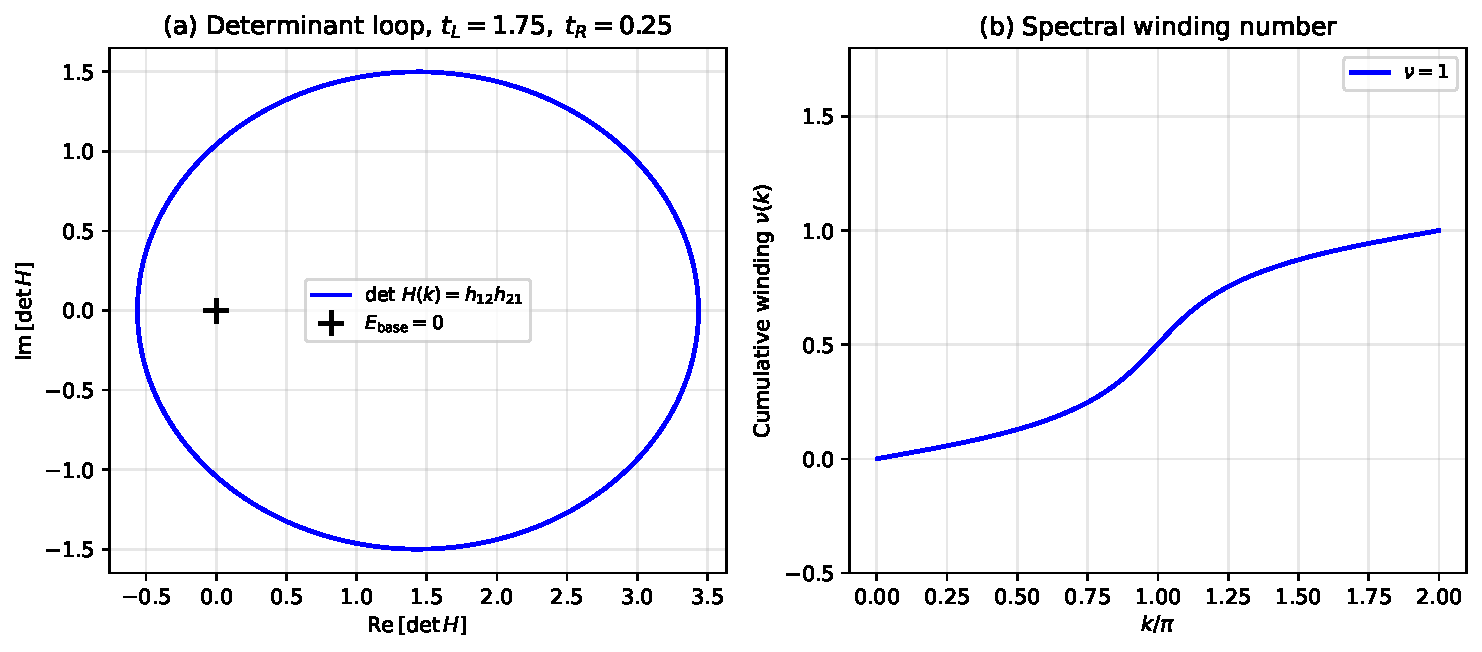
\includegraphics[width=0.85\linewidth]{figures/fig_f12_spectral_loop.pdf}
 \caption{Spectral winding number for the asymmetric-hopping NH SSH model
 ($t_L = 1.75$, $t_R = 0.25$, $t_2 = 1.0$).
 (a)~The determinant $\det H(k) = h_{12}(k)\,h_{21}(k)$ traces a loop in
 the complex plane that encircles the origin, confirming a point-gap
 topology with winding number $\nu = 1$.
 (b)~The cumulative winding accumulates smoothly from $0$ to $1$ as $k$
 traverses the Brillouin zone. Because $t_L > t_2 > t_R$, only $h_{21}$
 winds around the origin, producing a net spectral winding.}
 \label{fig:spectral-loop}
\end{figure}

\subsection{Physical meaning}
\label{ssec:winding-physical}

A nonzero winding number means the complex band forms a closed loop in
the complex $\omega$ plane that cannot be contracted to a point without
crossing $E_{\mathrm{ref}}$. This is the simplest example of a
topological invariant that exists \emph{only} in non-Hermitian systems:
a real-valued band confined to the real axis has zero winding around any
point off the axis.

In photonic crystals with complex $\epsr(\rr)$, the winding number
classifies point-gap topology of complex photonic bands. In one
dimension it is tied to the non-Hermitian skin effect under open
boundary conditions rather than to ordinary Hermitian edge-state
counting~\cite{zhong2021non}.

\subsection{Computational procedure}
\label{ssec:winding-computation}

The winding number~\eqref{eq:winding-number} is straightforward to
compute numerically:
\begin{enumerate}
 \item Sample $k$ uniformly on $[-\pi, \pi]$ with $N \gg 1$ points.
 \item Evaluate $\omega(k)$ from the Bloch eigenproblem (or from a
 tight-binding model).
 \item Form the shifted band $z(k) = \omega(k) - E_{\mathrm{ref}}$.
 \item Compute the total phase winding:
 $\wnum = [\arg z(\pi) - \arg z(-\pi)]/(2\pi)$, using the unwrapped
 phase.
 \item Alternatively, use the discrete winding formula:
 $\wnum = (2\pi)^{-1}\sum_{j=1}^{N}\arg[z(k_{j+1})/z(k_j)]$, which
 is gauge-invariant and numerically robust.
\end{enumerate}
The result is automatically an integer up to rounding errors.

\subsection{Example: Hatano--Nelson model}
\label{ssec:winding-hatano-nelson}

The Hatano--Nelson model (Chapter~\ref{ch:skin-effect}) provides a
minimal example. With asymmetric hopping $t_R \neq t_L$, the PBC band
structure is
\begin{equation}
 \omega(k) = t_R\,e^{ik} + t_L\,e^{-ik}.
 \label{eq:hn-band}
\end{equation}
This traces an ellipse in the complex plane with semi-axes
$|t_R + t_L|$ and $|t_R - t_L|$. When $t_R \neq t_L$, the ellipse has
nonzero area, and any point inside it has winding number
$\wnum = \pm 1$. Points outside the ellipse have $\wnum = 0$.

The physical consequence is striking: the OBC spectrum fills the
\emph{interior} of the PBC ellipse (see Chapter~\ref{ch:skin-effect}),
and all OBC eigenstates localize at one edge. The winding number
predicts this macroscopic spectral collapse.


%% ================================================================
\section{Biorthogonal Berry phase}
\label{sec:biorthogonal-berry}

In a non-Hermitian periodic system, the left and right Bloch eigenvectors
$\mathbf{u}_n^{\mathrm{L}}(\kk)$ and $\mathbf{u}_n^{\mathrm{R}}(\kk)$
are generally different (Section~\ref{sec:qnm-adjoint}). The Berry
connection must be generalized to a biorthogonal form:
\begin{equation}
 \Acal_n^{\mathrm{bi}}(\kk)
 = i\,\frac{\langle\mathbf{u}_n^{\mathrm{L}}(\kk)|\nabla_\kk|
 \mathbf{u}_n^{\mathrm{R}}(\kk)\rangle}
 {\langle\mathbf{u}_n^{\mathrm{L}}(\kk)|\mathbf{u}_n^{\mathrm{R}}(\kk)\rangle}.
 \label{eq:biorthogonal-berry}
\end{equation}
The biorthogonal Berry curvature and Chern number are defined analogously.
They reduce to the standard (Hermitian) definitions when the system is
Hermitian and left and right eigenvectors coincide.

\subsection{Complex-valued Berry phase}
\label{ssec:complex-berry}

Unlike the Hermitian Berry connection, which is real-valued (for a
single band), the biorthogonal Berry connection~\eqref{eq:biorthogonal-berry}
is generically complex. Its real and imaginary parts have distinct
physical meanings:
\begin{itemize}
 \item The \emph{real part} $\Re\Acal_n^{\mathrm{bi}}$ generalizes the
 Hermitian Berry connection and enters the semiclassical equations of
 motion for wave-packet dynamics.
 \item The \emph{imaginary part} $\Im\Acal_n^{\mathrm{bi}}$ is a new
 non-Hermitian contribution that describes the $\kk$-dependence of the
 mode non-orthogonality. It is related to the derivative of the
 Petermann factor with respect to $\kk$.
\end{itemize}

The Berry connection itself can be complex, but the first Chern number
of an isolated line-gapped band remains integer-valued when a smooth
biorthogonal basis exists over the Brillouin-zone torus. Exceptional
points or gap closings invalidate the construction rather than producing
a meaningful non-integer Chern number.

\paragraph{Example: biorthogonal Berry phase of the gain--loss
SSH model.}
For the gain--loss SSH model~\eqref{eq:gain-loss-ssh} with
$\gamma < 2t$ (the $\PT$-unbroken phase), the right eigenvector of the
lower band is
$|u^{\mathrm{R}}_-(k)\rangle = (1,\; -\omega_-(k)/[t(1+e^{ik})])^\transpose$
(up to normalisation). The left eigenvector is obtained by replacing
$H(k)$ with $H^\dagger(k)$. The biorthogonal Berry phase around the
Brillouin zone is
\begin{equation}
 \phi^{\mathrm{bi}} = \oint_{\BZ}
 \Acal_-^{\mathrm{bi}}(k)\;\dd k.
 \label{eq:biorthogonal-zak}
\end{equation}
For $\gamma = 0$ (Hermitian limit), this reduces to the standard Zak
phase: $\phi^{\mathrm{bi}} = \pi$ in the topological phase ($t' > t$)
and $\phi^{\mathrm{bi}} = 0$ in the trivial phase. As $\gamma$
increases, $\phi^{\mathrm{bi}}$ acquires an imaginary part that grows
continuously, but the real part remains quantized at $0$ or $\pi$ as
long as the chiral symmetry $\sigma_z H(k) \sigma_z = -H(k)$ is
preserved. At the $\PT$-breaking transition ($\gamma = 2t$), the
biorthogonal Berry phase is undefined because the denominator
$\langle u^{\mathrm{L}}_- | u^{\mathrm{R}}_- \rangle$ vanishes at the
EP.

\begin{figure}[t]
 \centering
 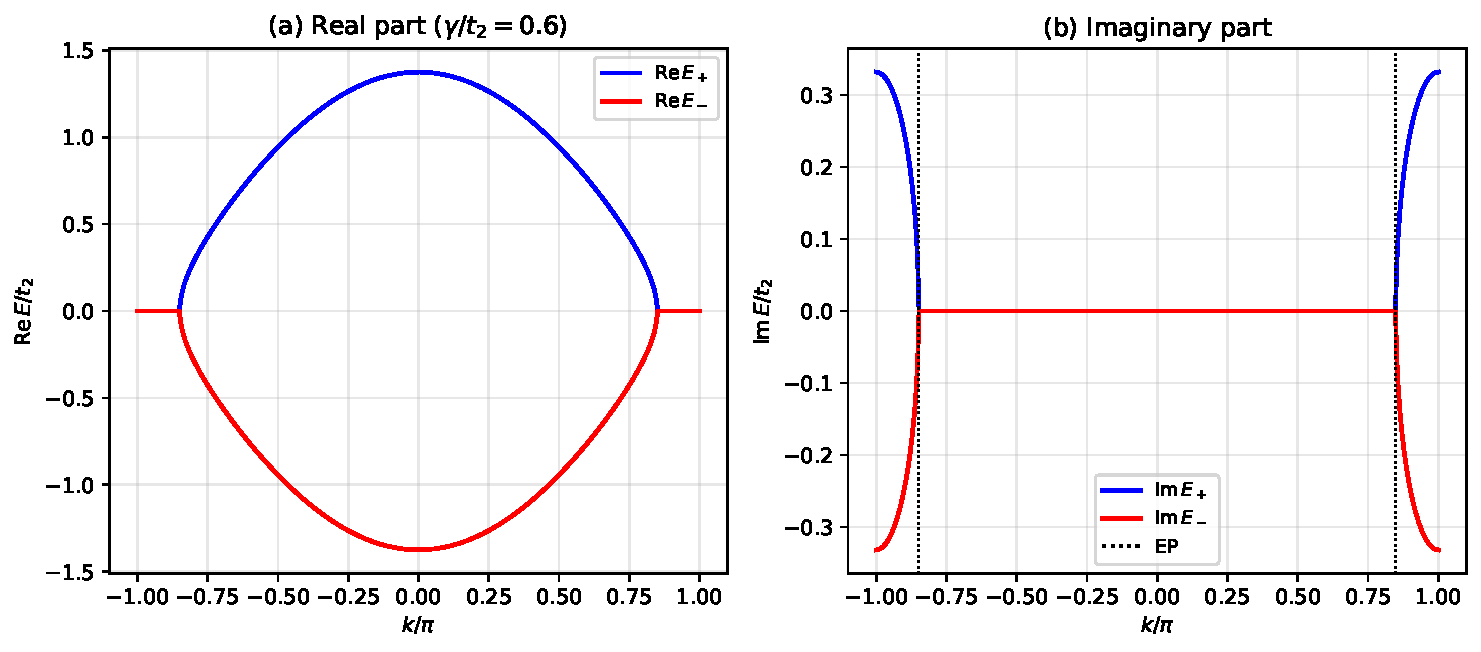
\includegraphics[width=0.85\linewidth]{figures/fig_f12_nhssh_bands.pdf}
 \caption{Complex band structure of the gain--loss SSH model
 ($t_1 = 0.5$, $t_2 = 1.0$, $\gamma/t_2 = 0.6$).
 (a)~Real part of the energy: the two bands touch near the exceptional
 points (dotted lines), where the square root in
 $E_\pm = \pm\sqrt{h_{12}h_{21} - \gamma^2}$ vanishes.
 (b)~Imaginary part: zero inside the $\PT$-symmetric region and
 bifurcating symmetrically in the $\PT$-broken region between the EPs,
 where one mode is amplified and the other is attenuated.}
 \label{fig:nhssh-complex-bands}
\end{figure}

This example illustrates a general principle: \emph{the real part of
the biorthogonal Berry phase is topologically protected by symmetry,
while the imaginary part is a smooth, non-topological measure of
non-Hermiticity.} The EP is the singularity where the Berry phase
becomes undefined---the non-Hermitian analogue of a gap closing in
Hermitian topology.

\subsection{Singularity at exceptional points}
\label{ssec:berry-ep}

Near an exceptional point, the denominator
$\langle\mathbf{u}_n^{\mathrm{L}}|\mathbf{u}_n^{\mathrm{R}}\rangle \to 0$
and the biorthogonal Berry connection diverges. This singularity reflects
the coalescence of eigenvectors and is intimately connected to the
topological charge of the EP (Section~\ref{sec:ep-topology}).

The Berry phase accumulated around a loop encircling an EP in the BZ is
$\pm\pi$ for an EP$_2$ (a $\pi$-Berry phase), analogous to the Berry
phase around a Dirac point in graphene. However, the non-Hermitian
version involves the biorthogonal inner product and does not require
time-reversal or inversion symmetry.


%% ================================================================
\section{Exceptional points in band structure}
\label{sec:ep-bands}

In a two-dimensional Brillouin zone, exceptional points appear as
isolated points in $\kk$-space where two complex bands touch. Near an
EP at $\kk_{\mathrm{EP}}$, the eigenvalue splitting follows the
square-root topology:
\begin{equation}
 \omega_\pm(\kk) \approx \omega_{\mathrm{EP}}
 \pm \sqrt{\alpha(\kk - \kk_{\mathrm{EP}})},
 \label{eq:ep-band-splitting}
\end{equation}
with $\alpha$ a complex coefficient. Encircling the EP in momentum space
exchanges the two bands---the same Riemann-surface structure as in
parameter-space encircling (Section~\ref{sec:encircling}).

\subsection{Exceptional lines and surfaces}
\label{ssec:ep-lines}

In three-dimensional systems or in systems with additional parameters,
EPs can form lines or surfaces in the combined $(\kk, \text{parameter})$
space. An \emph{exceptional ring} in a 2D BZ is a closed curve of EPs;
the interior of the ring and the exterior have different topological
indices.

In three-dimensional photonic crystals~\cite{chen2021ideal,pan2023real,liu2021observation}, exceptional points generically
form one-dimensional curves in the 3D BZ---\emph{exceptional lines}.
These lines are topological objects: they carry a topological charge
(a $\pi$ Berry phase for any loop encircling the line) and can be linked
or knotted with one another. The linking number is a topological
invariant that cannot change without two exceptional lines crossing.

\subsection{Bulk Fermi arcs}
\label{ssec:fermi-arcs}

When two complex bands are projected onto the real-frequency axis, the
regions where they overlap in $\Re\omega$ but differ in $\Im\omega$
create \emph{bulk Fermi arcs}---open arcs in the surface Brillouin zone
that connect projections of EPs. These arcs are a non-Hermitian
analogue of the Fermi arcs in Weyl semimetals~\cite{park2022nodal}, but they exist in the
bulk spectrum rather than at a surface.

The physical consequence is that constant-frequency cuts through the
complex band structure show open contours rather than closed Fermi
surfaces. This has been observed experimentally in photonic crystals
with controlled gain and loss~\cite{he2016acoustic,zhang2021acoustic}.

\paragraph{Observing bulk Fermi arcs in photonics.}
In a photonic crystal slab with $\PT$-symmetric gain and loss, bulk
Fermi arcs manifest as anomalous isofrequency contours in the
transmission spectrum. At a frequency where two complex bands overlap
in $\Re\omega$ but split in $\Im\omega$, an incident plane wave couples
to both bands with different decay rates. The transmitted intensity
shows a characteristic double-Lorentzian lineshape whose angular
dependence traces the Fermi arc in the surface Brillouin zone. The
arc endpoints are the projections of the bulk EPs, which can be located
by finding the angles at which the double Lorentzian degenerates into a
single peak with a squared-Lorentzian profile---the spectral signature
of an EP.

This measurement protocol requires only angle-resolved transmission
spectroscopy, making it accessible with standard photonic-crystal
characterization equipment. The main experimental challenge is
achieving sufficiently uniform gain--loss distribution across the
sample to resolve the Fermi-arc topology.


%% ================================================================
\section{The 38-fold classification}
\label{sec:classification}

\subsection{From tenfold to 38-fold}
\label{ssec:tenfold-to-38}

The full classification of non-Hermitian topological
phases~\cite{kawabata2019symmetry} extends the tenfold Altland--Zirnbauer
classification of Hermitian systems to 38 symmetry classes. The
expansion arises because:
\begin{enumerate}
 \item Non-Hermiticity distinguishes transposition from complex
 conjugation, doubling the number of anti-unitary symmetry classes.
 \item Both line gaps and point gaps must be considered independently.
 \item Sublattice symmetry and pseudo-Hermiticity become independent
 symmetry classes.
\end{enumerate}

Specifically, in Hermitian systems, time-reversal symmetry ($T$) and
particle-hole symmetry ($C$) are both anti-unitary and satisfy
$T H T^{-1} = H$ and $C H C^{-1} = -H$. In non-Hermitian systems,
transposition ($T^\top$: $H^\top = H$) and complex conjugation
($T^*$: $H^* = H$) are distinct symmetries because $H \neq H^\dagger$.
Similarly, $C^\top$ and $C^*$ become independent. This doubling of
symmetry types, combined with the two gap types, yields $38$ distinct
classes.

\subsection{Photonic symmetry classes}
\label{ssec:photonic-classes}

For the photonic systems that are our primary concern, the most relevant
symmetry classes and their topological invariants can be understood
through a few paradigmatic examples.

In one dimension with a point gap, the classification is $\mathbb{Z}$,
with the winding number~\eqref{eq:winding-number} as the topological
invariant. This is the symmetry class of the Hatano--Nelson model: the
asymmetric hopping breaks Hermiticity, opens a point gap, and the
resulting nonzero winding predicts the non-Hermitian skin effect. Any
one-dimensional photonic lattice with asymmetric coupling---whether from
non-reciprocal elements, spatially varying gain and loss, or
geometry-induced asymmetry---falls into this class.

In two dimensions with a line gap and broken time-reversal symmetry, the
classification is again $\mathbb{Z}$, but the invariant is the
biorthogonal Chern number of Chapter~\ref{ch:berry-maxwell}. This
generalizes the quantum Hall class to non-Hermitian systems: a magneto-optical
photonic crystal with uniform loss has complex bands separated by a line
gap, and the Chern number computed from the biorthogonal Berry
curvature correctly predicts the number of chiral edge states, even
though the edge-state frequencies are themselves complex.

Two-dimensional systems with a point gap support a different
$\mathbb{Z}$ invariant: a two-dimensional winding number that
characterizes how the complex spectrum wraps around the reference point
as $\kk$ sweeps the Brillouin zone. This invariant predicts the
two-dimensional non-Hermitian skin effect, where bulk states localize
at corners of a finite sample rather than at edges.

Finally, one-dimensional systems with $\PT$ symmetry and a line gap are
classified by $\mathbb{Z}_2$: a quantized Zak phase that takes values
$0$ or $\pi$. This is the non-Hermitian analogue of the Su--Schrieffer--Heeger
topological insulator, and the $\mathbb{Z}_2$ invariant correctly
predicts the presence or absence of $\PT$-symmetric edge states.

\paragraph{Example: symmetry-class identification for the
gain--loss SSH model.}
The systematic procedure for identifying the symmetry class of a
concrete non-Hermitian photonic system is as follows. We illustrate
each step using the gain--loss SSH model~\eqref{eq:gain-loss-ssh},
whose Bloch Hamiltonian is
$H(k) = (t_1 + t_2 \cos k)\,\sigma_x + t_2 \sin k\,\sigma_y
+ i\gamma\,\sigma_z$.

\emph{Step 1.} Write the Bloch Hamiltonian $H(\kk)$ from the Maxwell
eigenproblem. For the gain--loss SSH model, this is the $2\times 2$
matrix above with two sublattice degrees of freedom.

\emph{Step 2.} Check for time-reversal symmetry. We need
$H(\kk) = H^*(-\kk)$. Since the hopping amplitudes $t_1$, $t_2$ are
real and $i\gamma$ is purely imaginary, we find
$H^*(-k) = (t_1 + t_2\cos k)\,\sigma_x - t_2\sin k\,\sigma_y
- i\gamma\,\sigma_z$. This equals $H(k)$ only if $\gamma = 0$, so
$T^*$ symmetry is broken by the gain--loss. However, transposition
symmetry $H(k) = H^\top(-k)$ \emph{is} present because $\sigma_x$ and
$\sigma_z$ are symmetric and $\sigma_y$ is antisymmetric, and the
$\sigma_y$ coefficient is odd in $k$. This is the non-Hermitian
generalization of time-reversal for spinless particles.

\emph{Step 3.} Check for $\PT$ symmetry: $\sigma_x H(k)\sigma_x = H^*(-k)$
can be verified by direct computation. The $\sigma_x$ operator
interchanges the two sublattices (gain and loss sites), while complex
conjugation reverses the sign of $i\gamma$. Thus $\PT$ symmetry is
present, corresponding to pseudo-Hermiticity $\eta H \eta^{-1} = H^\dagger$
with $\eta = \sigma_x$.

\emph{Step 4.} Check for chiral (sublattice) symmetry:
$\sigma_z H(k) \sigma_z = -H(k)$. Direct computation confirms this:
$\sigma_z \sigma_x \sigma_z = -\sigma_x$,
$\sigma_z \sigma_y \sigma_z = -\sigma_y$, and
$\sigma_z (i\gamma\sigma_z) \sigma_z = i\gamma\sigma_z$. Wait---the
last term gives $+i\gamma\sigma_z$, not $-i\gamma\sigma_z$. So
standard chiral symmetry is broken by the gain--loss. However, a
\emph{non-Hermitian} chiral symmetry $\sigma_z H(k) \sigma_z = -H^\dagger(k)$
\emph{is} present, because $H^\dagger(k)$ flips the sign of
$i\gamma\sigma_z$.

\emph{Step 5.} Cross-reference with the 38-fold table. The combination
of transposition symmetry $T^\top$ with $(T^\top)^2 = +1$, non-Hermitian
chiral symmetry, and pseudo-Hermiticity places the system in class
BDI$^\dagger$ with a point gap. The table entry for BDI$^\dagger$ in
one dimension with a point gap is $\mathbb{Z}$: the topological
invariant is the winding number, consistent with the spectral-loop
analysis of Section~\ref{ssec:1d-example}.

\subsection{Reduction to the Hermitian tenfold way}
\label{ssec:hermitian-reduction}

The 38-fold classification must reduce to the standard tenfold
Altland--Zirnbauer classification when the Hamiltonian is Hermitian.
This consistency check is instructive. When $H = H^\dagger$:
transposition symmetry $H = H^\top$ becomes equivalent to complex
conjugation $H = H^*$ (since $H^\top = H^{\dagger *} = H^*$), so the
doubling of anti-unitary symmetries collapses. The point gap becomes
trivially satisfied (the spectrum is real and generically does not pass
through any complex reference point), so point-gap invariants become
trivial. Only line-gap invariants survive, and they coincide with the
standard band-gap invariants. The $38$ classes collapse to $10$, and
the topological periodic table reduces to the familiar Kitaev table.

For the gain--loss SSH model, taking $\gamma \to 0$ restores Hermiticity.
The BDI$^\dagger$ class collapses to the Hermitian BDI class, and the
$\mathbb{Z}$ winding number reduces to the standard winding number of
the SSH model. The point-gap topology becomes trivial (the spectrum
is real and does not wind around any complex point), and only the
line-gap $\mathbb{Z}$ invariant---the Zak phase---survives. This
continuity between non-Hermitian and Hermitian classifications is
essential for physical consistency: the topological properties of a
photonic crystal with weak gain and loss must continuously deform into
those of the passive structure.

\subsection{Beyond the periodic table}
\label{ssec:beyond-table}

The 38-fold classification is a bulk classification that applies to
infinite periodic systems. Several features of real photonic structures
lie outside its scope:
\begin{itemize}
 \item Finite-size effects modify the spectrum and can change the
 topological phase.
 \item Disorder can stabilize or destroy non-Hermitian topological
 phases, depending on the symmetry class.
 \item The classification assumes a single-particle (quadratic)
 Hamiltonian; nonlinear and many-body effects require separate
 analysis (Chapter~\ref{ch:open-problems}).
 \item The Maxwell operator has additional structure (vector nature,
 gauge redundancy, frequency-dependent material response) that is
 not fully captured by the tight-binding classification. Lifting the
 38-fold table to continuous Maxwell operators is an open problem
 (Section~\ref{sec:maxwell-synthesis}).
\end{itemize}

\begin{takeaway}[Non-Hermitian topology requires new invariants]
The topological classification of Hermitian systems---Chern numbers,
$\mathbb{Z}_2$ indices, winding numbers of real bands---is insufficient
for non-Hermitian photonics. Complex bands, point gaps, spectral winding,
and biorthogonal Berry phases introduce genuinely new topological
structures. These structures predict phenomena---the skin effect,
anomalous edge states, bulk Fermi arcs---that have no Hermitian analogue.
\end{takeaway}
